\chapter{Data}\label{data}

A crucial part of every analysis are the data. To be able to conduct an analysis with results that can reasonably represent the domain, we need to have enough of them - the more the better. 

Our dataset consist of 658,460 song lyrics scraped from the crowd-sourced website 
Genius\footnote{\url{https://genius.com/}}. Sadly, the original author of the dataset is unknown, it has been passed on to us by a colleague as a potentially interesting source for research. However, all song lyrics are publicly available on the Genius website and can be linked with the corresponding item of the dataset via the \textit{url} attribute.

We apologize for any strong language that may be used in song lyrics or their excerpts in this thesis. Due to its various forms and the size of the dataset, it would be extremely difficult to remove them, and because they occur in pop culture naturally, we chose to portray them faithfully.

\section{Preprocessing}

In most areas it is very hard to find a dataset of good quality and large quantity. Usually at least one of the two suffers. It is not any different with our data - although the dataset is large, the contents were created by ordinary people and intended for human readers so they are not well suited for automated processing. It is necessary to look closely at the data, remove faulty or redundant items, and clean the rest with preprocessing.

To assess what are the problems in the data and how to address them, we created a very small dataset of only about 10 songs which we cleaned manually. To select these songs, we looked at about 100 random songs and chose the ones that contained the most common faults. We also tried to contain a broad spectrum of errors by focusing on the diversity in the selected dataset. We then iteratively implemented an automated solution for each type of data corruption, comparing the automatically and manually cleaned data, until they matched. We also extracted statistical information that further showed the weak points that needed addressing.

We received the dataset in JSON format, with each song as a separate item, each containing following features:

\begin{itemize}
	\item \textit{title} - the name of the song
	\item \textit{lyrics} - the text of the song's lyrics
	\item \textit{album} - song's album (or null)
	\item \textit{genre} - one of the following: rap, pop, rock, r-b, country
	\item \textit{artist} - song's performer
	\item \textit{url} - the url of the lyrics page on Genius website
	\item \textit{year} - the year the song was produced
	\item \textit{is\_music} - boolean flag distinguishing song lyrics from other texts
	\item other song details: \textit{producer, featured artist, recording location, charts, writer, samples, sampled in, has featured video, has featured annotation}
	\item other website specific information: \textit{rg artist id, rg type, rg tag id, rg song id, rg album id, rg created, has verified callout}	
\end{itemize}

The features from the last two points were \textit{null} for all or most of the items. That, and the fact that they do not give us much more information that would contribute to the lyrics analysis, made them useless and so we decided not to keep them. We removed all songs for which the attribute \textit{is\_music} was False, indicating it was not a song (often a poem or prose) or they did not contain lyrics - 34,259 songs in total. We further removed one song with invalid (incomplete) JSON. After comparing the lyrics to each other, we found and removed 32,551 duplicates.

Upon further inspection, we found out that our dataset also contains lyrics in different languages. We used the neural network model for language identification by Google (CLD3)\footnote{\url{https://github.com/google/cld3}} for the classification. It showed that our dataset contains exactly 100 different languages, most of them represented only marginally. Since other languages did not have enough data to support a good analysis and implementing them would be above the scope of this thesis, we kept only English lyrics. We further removed 832 items with language detection errors. All of them were under 10 lines long so they would not be a valuable addition anyway. At this point our dataset contained 438,037 items.

\begin{figure}[!htb]
	\minipage{0.49\textwidth}
	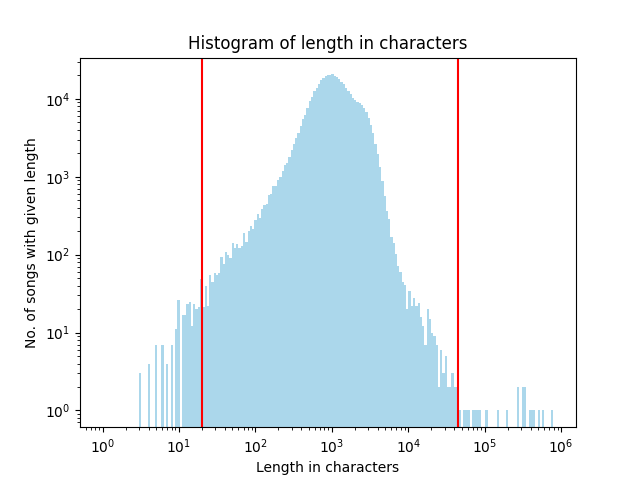
\includegraphics[width=\linewidth]{../img/histogram_song_length_in_char.png}
	\caption{Histogram of number of characters in songs of our dataset.}\label{hist_chars}
	\endminipage\hfill
	\minipage{0.49\textwidth}
	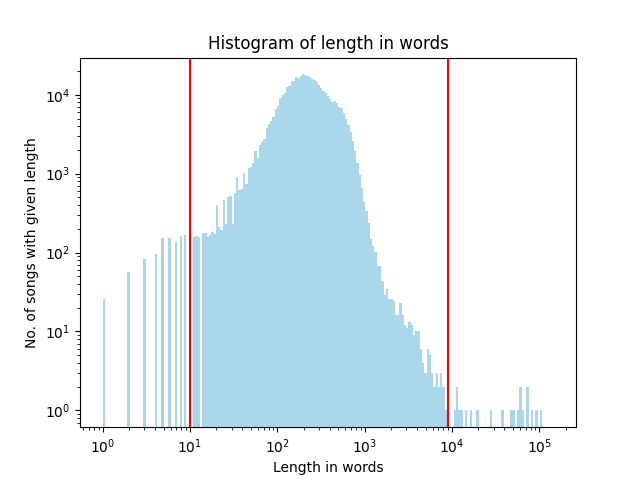
\includegraphics[width=\linewidth]{../img/histogram_song_length_in_words.png}
	\caption{Histogram of number of words in songs of our dataset.}\label{hist_words}
	\endminipage\hfill
	
\end{figure}
\begin{figure}[!h]\centering
	\minipage{0.49\textwidth}
	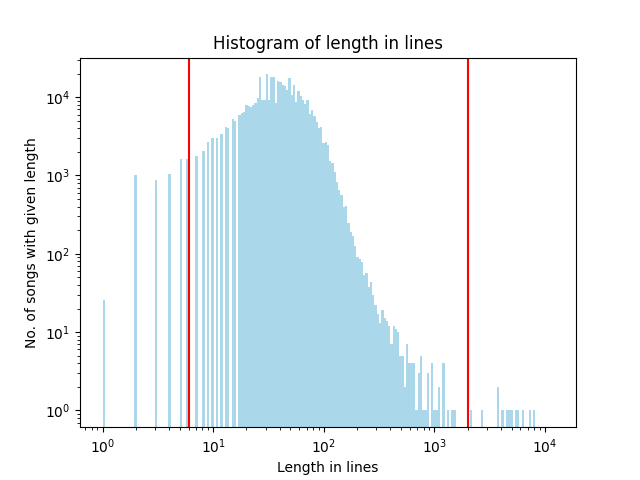
\includegraphics[width=\linewidth]{../img/histogram_song_length_in_lines.png}
	\caption{Histogram of number of lines in songs of our dataset.}\label{hist_lines}
	\endminipage\hfill
\end{figure}

To learn more about our data, we created histograms with song's length in characters, words, and lines (see Figures \ref{hist_chars}, \ref{hist_words}, \ref{hist_lines}). Knowing the common issues of extreme values, we manually examined a few of the shortest and a few of the longest items. Confirming our expectations, we found out that they were not valid songs either. The long ones were usually book excerpts or rap improvisation battles, while the short ones were often links to advertisements or motivational quotes. We removed 14 long and 1,838 short lyrics. Although it may not seem as much, it could have strong negative influence mainly during the generation phase. In Figures \ref{hist_chars}, \ref{hist_words}, and \ref{hist_lines}, red lines mark the borders for removal - only the items in between them were kept.


\section{Structure of the data}

This section gives statistical information about the dataset after preprocessing. Table \ref{basic_stats} sums up basic statistics about the data overall and for each genre specifically. Pie chart in Figure \ref{piechart_genres} shows the portions of the data belonging to each genre. All the attributes are listed in Table \ref{stats_nonempty_values}. For some songs, not all attributes are available. Number of items for with non-empty values is given as well.
\begin{table}[h!]
	\centering
	\begin{tabular}{c | r r r} 
		Genre & Songs & Avg. lines per song & Avg. words per line \\ 
		\midrule \midrule
		Pop & 293,679& 36.73 & 5.50\\
		Rap & 99,189 & 64.32 & 6.88 \\
		Rock & 34,372 & 38.73 & 5.30 \\
		R\&B & 5,126 & 52.82 & 5.51 \\
		Country & 3,819 & 38.43 & 5.85 \\
		\midrule
		Total & 436,185 & 43.36 & 5.96 \\
	\end{tabular}
	\caption{Basic statistics about the dataset.}
	\label{basic_stats}
\end{table}



\begin{figure}[h]\centering
	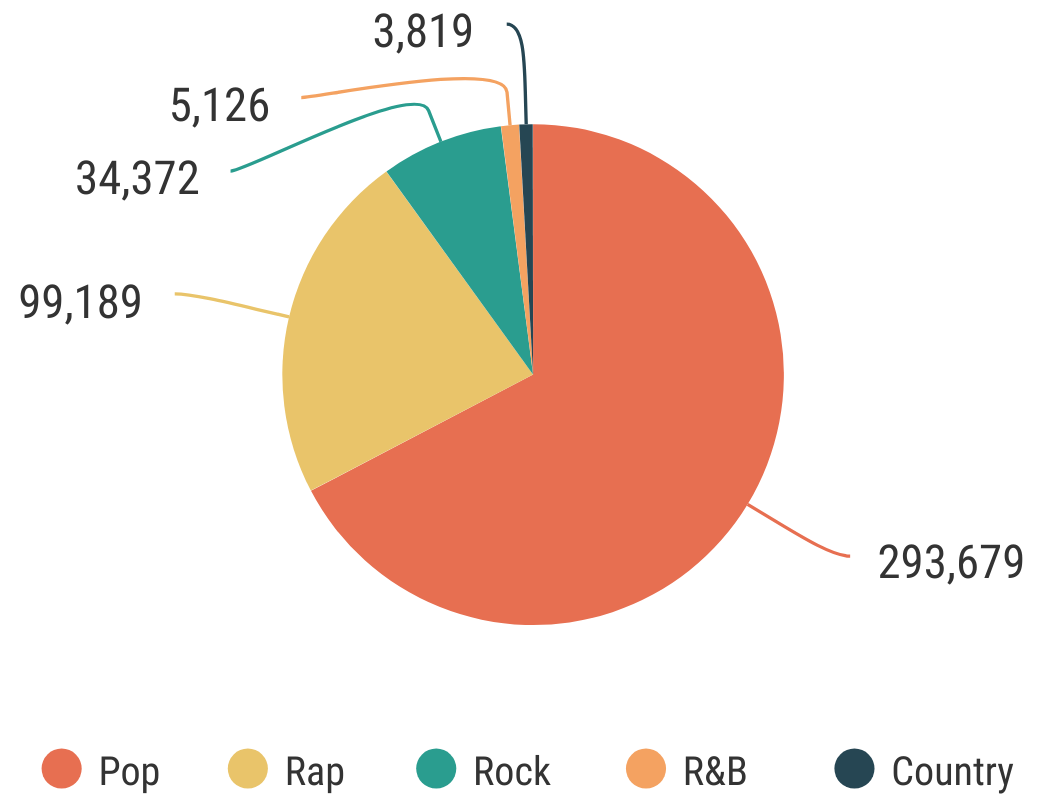
\includegraphics[scale=0.25]{../img/piechart_genres.png}
	\caption{Distribution of genres in the dataset.}\label{piechart_genres}
\end{figure}



\begin{table}[h!]
	\centering
	\begin{tabular}{| c | r |} 
		\hline
		Attribute & Non-empty values \\ [0.5ex] 
		\hline
		lyrics & 436,185 \\
		title & 436,179 \\
		album & 112,060 \\
		genre & 436,185 \\ 
		artist & 436,184 \\ 
		url & 436,185 \\
		year & 96,491 \\ 
		lang & 436,185 \\
		id & 436,185 \\
		word\_count & 436,185 \\
		\hline
	\end{tabular}
	\caption{Attributes and their counts of non-empty values.}
	\label{stats_nonempty_values}
\end{table}

\section{Annotated subset}
From the dataset described above, we separated a subset of 50 songs, 10 song for each genre, and annotated them with rhyme schemes ourselves. We then separated them into a development and test set, so that both groups would have an approximately equal number of non-empty lines per genre (plus or minus 2 lines). We reserved the development set for iterative testing and improvement of our algorithm. The test set was used as an additional checkpoint for final evaluation, as you can read in Chapter \ref{evaluation}.

\section{Chicago Rhyming Poetry Corpus}
For an additional dataset for evaluation, we included one from an outside source -- the Chicago Rhyming Poetry Corpus\footnote{\url{https://github.com/sravanareddy/rhymedata}}, annotated with rhyme schemes by professionals. It contains 1,321 poems from 32 authors written in 14\textsuperscript{th} to 19\textsuperscript{th} century. It has a total of 93,045 lines with an average of 70.44 lines per song. It is the same dataset that was used for training and evaluation of Rhyme Tagger.



